\documentclass[11pt, a4paper]{article}

\usepackage[left=2cm, top=3cm, text={17cm, 24cm}]{geometry}
\usepackage{times}
\usepackage{amsfonts}
\usepackage{graphicx}
\usepackage{hyperref}
\usepackage{float}
\usepackage[czech]{babel}
\begin{document}

\begin{center}


\Huge
\textsc{Fakulta informačních technologií\\
Vysoké učení technické v~Brně}
\\[84mm]
\Huge \textbf{Webové aplikace -- 2. projekt}\\
\LARGE{Implementační dokumentace}\\
\LARGE  Tým 08 -- Organizátor schůzek\\
\vspace{\stretch{9.5}}
\end{center}

\hfill


%%% Names %%%
\begin{minipage}[l]{0.6 \textwidth}
\Large
\begin{tabular}{l l}
\textbf{Lukáš Havlíček} & \textbf{(xhavli46)}\\
Jakub Sadílek & (xsadil07)\\
Jaroslav Katrušák & (xkatru00)\\
Filip Weigel & (xweige01)\\
\end{tabular}
\end{minipage}

\thispagestyle{empty}
\clearpage
\setcounter{page}{1}

\section{Zadání}
Implementujte webovou aplikaci vhodnou pro organizaci schůzek a jiné domlouvání termínů událostí (akcí). Aplikace umožní libovolnému návštěvníkovi vygenerovat novou událost (akci). Uživatel bude mít možnost vytvořit několik alternativních termínů konání události (akce), např. podle dnů, nebo hodin. Aplikace by uživateli měla umožnit automaticky generovat termíny podle zadaných kritérií (např. každou celou hodinu v pracovní době uvedených dnů, pracovní dobu stanovuje uživatel).\\

Aplikace pro nově vytvořenou událost vygeneruje náhodný řetězec (řetězce) o vhodné délce pomocí kterého bude možné podávat organizátorovi události zpětnou vazbu k termínu události a prohlížet výsledky. Aplikace vygeneruje URL obsahující výše uvedené řetězce pro snadný přístup k hlasování a výsledkům hlasování.\\

Očekává se, že organizátor akce bude výše uvedené URL distribuovat zájemcům o aukci vlastními silami mimo implementovanou aplikaci.\\

Aplikace automaticky smaže všechna data k události 14 dnů po nastaveném termínu konání akce.

\section{Implementace}
Projekt je implementován v jazycích HTML, PHP a Javascript. Frondend je implementován pomocí CSS a frameworku Bootstrap.
\subsection{Backend}
Úvodní stránka je implementována v souboru \texttt{index.php}. Manuálně si lze přidat termín, nebo lze termín generovat automaticky podle zvolených kritérií, kterými jsou počáteční datum a čas, a koncový datum a čas včetně rozestupů mezi jednotlivými termíny. Dále při automatickém generování lze zvolit pro které dny v týdnu si přeje uživatel generovat termíny. Standartně jsou zvoleny pracovní dny v týdnu.\\

Automatické generování termínu je implementováno pomocí cyklů \texttt{for}. Nejdřive je pomocí cyklu zjištěno, které dny jsou vybrány pro automatické generování a poté následuje druhý cyklus, který postupně od počátečního času k času koncovému generuje termíny s požadovaným rozestupem.\\

Po vygenerování termínu (manuálně/automaticky) se uživateli termíny zobrazí. Nevyhovující termíny lze editovat, nebo odebrat. Odebrání a editace termínu je realizována pomocí \texttt{javascriptu}, při kterém je využito i \texttt{jquery} pro výběr prvků z samotné stránky. Poté je nutné vyplnit název události a následně je možné vygenerovat událost pomocí tlačítka \texttt{založit hlasování}. 
Backend přijme informace o události a termínech, přidělí ji \texttt{ID}, vytvoří nové záznamy v databázi událostí a termínů k dané události. \\

\texttt{hlasovani.php?id=x}, kde \texttt{x} je \texttt{ID} události. Na tento \texttt{link} je uživatel přesměřován po založení hlasování. Backend dle požadavku GET vybere termíny z dané události a termíny jsou zobrazeny uživateli. Uživatel může zvolit termíny, pro které chce hlasovat - implementovány pomocí \texttt{checkboxu} - a odešle je pomocí metody \texttt{POST}. Následně backend \texttt{POST} přijme a pro každý zvolený termín inkrementuje v databázi počet hlasů o jeden hlas. Stejnému uživateli je zamezeno hlasovat vícekrát pro danou událost.\\

Pro uživatele není hlasování povinné a pokud si nepřeje hlasovat, může se rovnou podívat na výsledky hlasování pomocí tlačítka \texttt{Výsledky}. Po stisknutí tlačítka je uživatel přesměřován na \texttt{vysledky.php?id=x}, kde \texttt{x} je \texttt{ID} události, backend pomocí metody \texttt{GET} dostane informace o požadované události a obratem zobrazí uživateli aktuální výsledky.  

\subsection{SQL databáze}
Databáze je implementována v jazyce SQL. Skript pro vytvoření databáze je obsažen ve souboru \texttt{SQL.txt} a konfigurace pro připojení k databázi je obsažena v souboru \texttt{config.php}. Databáze se skládá ze dvou tabulek. První tabulka \texttt{Schuzky}, která obsahuje primární klíč \texttt{SchuzkaID}, dále název schůzky a datum smazání schůzky (14 dní po uplynutí schůzky). Mazání je realizováno pomocí databázového \texttt{eventu}. Druhá tabulka obsahuje vygenerované termíny k právě jedné schůzce. Je složena z \texttt{TerminID}, který je primárním klíčem, časem pro daný termín, dále počtem hlasů a cizím klíčem \texttt{SchuzkaID}, který odkazuje do tabulky \texttt{Schuzky}. Při smazání schůzky dojde k automatickému smazání všech termínů, které byly se schůzkou provázány pomocí \texttt{on delete cascade} 

\begin{figure}[H]
\begin{center}
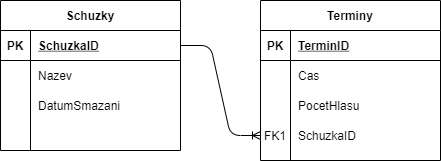
\includegraphics[scale=0.6]{dbDiagram.png}
\caption{Schéma SQL databáze}
\label{obr1}
\end{center}
\end{figure}
\subsection{Frontend}
Frontend je implementován pomocí HTML a pro vzhled je použit \texttt{css} předpis, který se nachází v souboru \texttt{style.css}. V souboru \texttt{style.css} jsou specifikovány barvy, velikosti písma, barvy písma a podobně. Rozložení stránky je řešeno pomocí frameworku \texttt{bootstrap} ve verzi 4.3.1 a pro jeho správnou funkcionalitu je třeba mít nalinkovaný \texttt{javascript} ve verzi 5.0.0 a výše. \texttt{Bootstrap} byl zvolen z důvodu rychlé realizace rozložení stránky a taktéž protože jsme se s ním mohli setkat i v jiných projektech. Frontend je implementován v souborech \texttt{index.php}, \texttt{hlasovani.php} a \texttt{vysledky.php}. 

\section{Závěr}
Při vypracovávání projektu jsme nenarazili na žádné větší obtíže. Komunikace probíhala pomocí serveru \texttt{Discord}, na kterém mohl každý člen diskutovat řešení projektu a připomínky k projektu. Pro verzování projektu jsme zvolili server \texttt{Github} \footnote{www.github.com/filaseek/wap}. V projektu se podařilo splnit všechny požadavky zadání a projekt lze tedy považovat za úspěšně dokončený. vypracovaný projekt je dostupný na \footnote{http://www.stud.fit.vutbr.cz/~xhavli46/wap/} a \footnote{http://www.wap.borec.cz/}

\end{document}

